%!xelatex = 'xelatex --halt-on-error %O %S'

\documentclass{buaaemp}
\newcommand{\sFeCl}[1]{\tup{FeCl\textsubscript{#1}}}
\newcommand{\sHIIO}{\tup{H\textsubscript{2}O}}
\newcommand{\specWaterPlus}{\,\sHIIO\,(\sFeCl3)\,}
\usepackage{cite}

\begin{document}

% 标题,作者
\emptitle{连续波核磁共振}
\empauthor{智朝晖}{钱建强}

% 奇数页页眉 % 请在这里写出第一作者以及论文题目
\fancyhead[CO]{{\footnotesize 智朝晖: 连续波核磁共振}}


%%%%%%%%%%%%%%%%%%%%%%%%%%%%%%%%%%%%%%%%%%%%%%%%%%%%%%%%%%%%%%%%
% 关键词 摘要 首页脚注
%%%%%%%%关键词
\Keyword{核磁共振\quad $g$因子\quad 弛豫时间\quad 尾波}
\twocolumn[
\begin{@twocolumnfalse}
\maketitle

%%%%%%%%摘要
\begin{empAbstract}
实验首先得到了掺有 \sFeCl3 的 \sHIIO 样品中质子的核磁共振信号,由此验证了核磁共振现象;并在此基础上考察了不同实验条件对核磁共振信号的影响。
	
	在此基础上,实验中利用\specWaterPlus 样品质子共振信号和质子回旋频率的参考值对永久磁铁的磁场进行了校准;并进一步利用校准后的磁场测定了氟核的$g$因子。
	此外,通过估测信号的半宽度$\Delta\omega$, 估测了聚四氟乙烯中氟核的横向弛豫时间。
\end{empAbstract}

%%%%%%%%首页角注,依次为实验时间、报告时间、学号、email
\empfirstfoot{2022-09-15}{2022-9-16}{20377365}{20377365@buaa.edu.cn}
\end{@twocolumnfalse}
]
%%%%%%%%!首页角注可能与正文重叠,请通过调整正文中第一页的\enlargethispage{-3.3cm}位置手动校准正文底部位置:
%%%%%%%%%%%%%%%%%%%%%%%%%%%%%%%%%%%%%%%%%%%%%%%%%%%%%%%%%%%%%%%%
%  正文由此开始
\wuhao 
%  分栏开始

\section{引~~言}
\subsection{原子核的基本特性}

原子由原子核和核外运动的电子所组成。原子核的基本性质有其电荷、质量、成分、大小、角动量和磁矩。原子核带正电,所带电量和核外电子的总电量相等,数值上等于最小电量单位$e$(1.6021$\times $10$^{-19}$C)的整数倍,称为电荷数。原子核的质量一般用质量数表示,接近于原子质量单位(1.66055 $\times $10$^{-27}$kg)的整数倍。原子核由质子和中子所组成。质子和中子的质量大致相等,但每个质子带正电量$e$,而中子则不带电。因此,元素周期表中的原子序数$Z$在数值上等于相应原子核外的电子数、核内质子数和核的电荷数。原子核的半径为10$^{-15}$m的数量级。

原子核具有本征角动量,等于核内所有轨道和自旋运动的角动量的总和。核自旋可用自旋量子数I来表征。核内的中子和质子都是$I$=1/2的粒子。实验证明,如将原子核按其自旋特性来分类,则可分为三类:(1)电荷数(即原子序数)与质量数都为偶数的核,如$^{12}$C,$^{18}$O)等,它们的自旋量子数为零;(2)质量数为单数的核,如$^1$H,$^{13}$C,$^{15}$N等,它们的自旋量子数为半整数(1/2,3/2,5/2);(3)质量数为双数,但电荷数(原子序数)为单数的核,$^2$H,$^{14}$N等,它们的自旋量子数为整数(1,2,3,...)。
\newpage

根据量子力学,一自旋量子数$I\neq0$的孤立原子核应具有本征自旋角动量$P_I$和本征自旋磁矩$\mu_I$:

$$P_I=\sqrt{I(I+1)\hbar},\mu_I=g_l\sqrt{I(I+1)\mu_N},$$

$P_I$和$\mu_I$方向互相平行。式中,$g_I$为原子核的朗德分裂因子,即$g$因子,其值随原子核的不同而不同。$\mu_N=\frac{e\hbar}{2M_P}=5.050824\times 10^{-27}\text{J/T}$,称为核磁子,是核磁矩的单位。这里的$e$和$M_P$分别是质子的电荷与质量。和电子磁矩的单位——玻尔磁子$\mu_B$相比($\mu_B=\frac{e\hbar}{2m_e}=9.204078\times 10^{-24}\text{J/T}$,$e$和$m_e$分别是电子的电荷和质量),因为电子质量仅为质子质量的1/1360,可知$\mu_B$比$\mu_N$要大得多,因而,电子磁矩也要比原子核磁矩大得多。原子核的磁矩可正可负,例如经测定,以$\mu_N$为单位,中子($^1$n,$I=1/2$)和$^{17}$O的磁矩都为负值,分别为-1.9130和-1.8930,而质子($^{1}$H,$I=1/2$)和$^{13}\text{C}$,$I=1/2$的磁矩均为正值,分别为2.7927和0.7022。

现在,设想一原子核位于沿$z$方向施加的恒定磁场$H_0$中,由于空间量子化,$P_I$和$\mu_I$沿$z$方向的分量$P_z$,$\mu_z$只能取一系列不连续的值:
$$P_z=m\hbar,$$
$$\mu_z=\gamma'P_z=m\gamma'\hbar.$$
式中,$\gamma'$是核磁矩和核自旋角动量之比,称为核的旋磁比;$m$是磁量子数,可取$I$,$I-1$,$I-2$,...,$-I+1$,$-I$等共$2I+1$个不连续的值。

应该指出,人们通常所说的原子核的角动量和磁矩指的是$P_z$,$\mu_z$的最大值,即
\begin{align*}
    P&=(P_z)_\text{max}=I\hbar \\
    \mu&=(\mu_z)_\text{max}=\gamma'I\hbar
\end{align*}


\subsection{核磁共振的经典物理描述}

从经典物理的观点看,如果定义单位体积内原子核磁矩的矢量和磁化强度为$\mathbf{M}$,则当该原子核系统位于恒定磁场中时,$\mathbf{M}$将以一定的角速度围绕磁场轴作拉莫(Lamor)进动并最终沿磁场方向取向。如图\ref{Fig1}(a)所示,这一过程涉及外加磁场作用下的自旋动力学问题。根据刚体转动力学原理,一绕自身轴转动的刚体(如陀螺)在受到一外力矩作用时,该刚体除了自身转动外,其自转轴还会绕着外力方向作进动。将原子核自旋系统与这种刚体的行为作类比,可以容易地写出无阻尼振动的理想情况下,该系统的角动量随时间的变化率应等于外加的磁场力矩,即
$$\frac{{\rm d}\mathbf{P}}{{\rm d}t}=\mu_0\mathbf{M}\times \mathbf{H}.$$
考虑到$M=\gamma'P$,可得原子核磁矩的进动方程为
$$\frac{{\rm d}\mathbf{M}}{{\rm d}t}=\gamma\mathbf{M}\times \mathbf{H}.$$
式中,$\gamma=\mu_0\gamma'=\frac{\mu_0eg_I}{2M_N}$表示核的磁偶极矩与自旋角动量比值的旋磁比。$\mu_0$和$M_N$分别是真空磁导率($\mu_0=4\pi\times 10^{-7}\text{H/m}$)和核的质量。核磁矩的进动图像如图\ref{Fig1}(a)所示,${\rm d}\mathbf{M}/{\rm d}t$垂直于$\mathbf{M}-\mathbf{H}$平面,使$\mathbf{M}$绕$\mathbf{H}$进动。

设在${\rm d}t$时间内$\mathbf{M}$从点$A$进动到点$B$,相应的$\theta$角保持不变,而在$x-y$平面内角度改变${\rm d}\varphi$,从图中几何关系可知${\rm d}M=\overline{AB}=M\sin\theta{\rm d}\varphi$,由此可得$\mathbf{M}$的拉莫进动频率为
$$\omega=\frac{{\rm d}\varphi}{{\rm d}t}=\frac{1}{M\sin\theta}\frac{{\rm d}M}{{\rm d}t}=\frac{\gamma MH\sin\theta}{M\sin\theta}=\gamma H.$$

\begin{figure}[H]
\centering
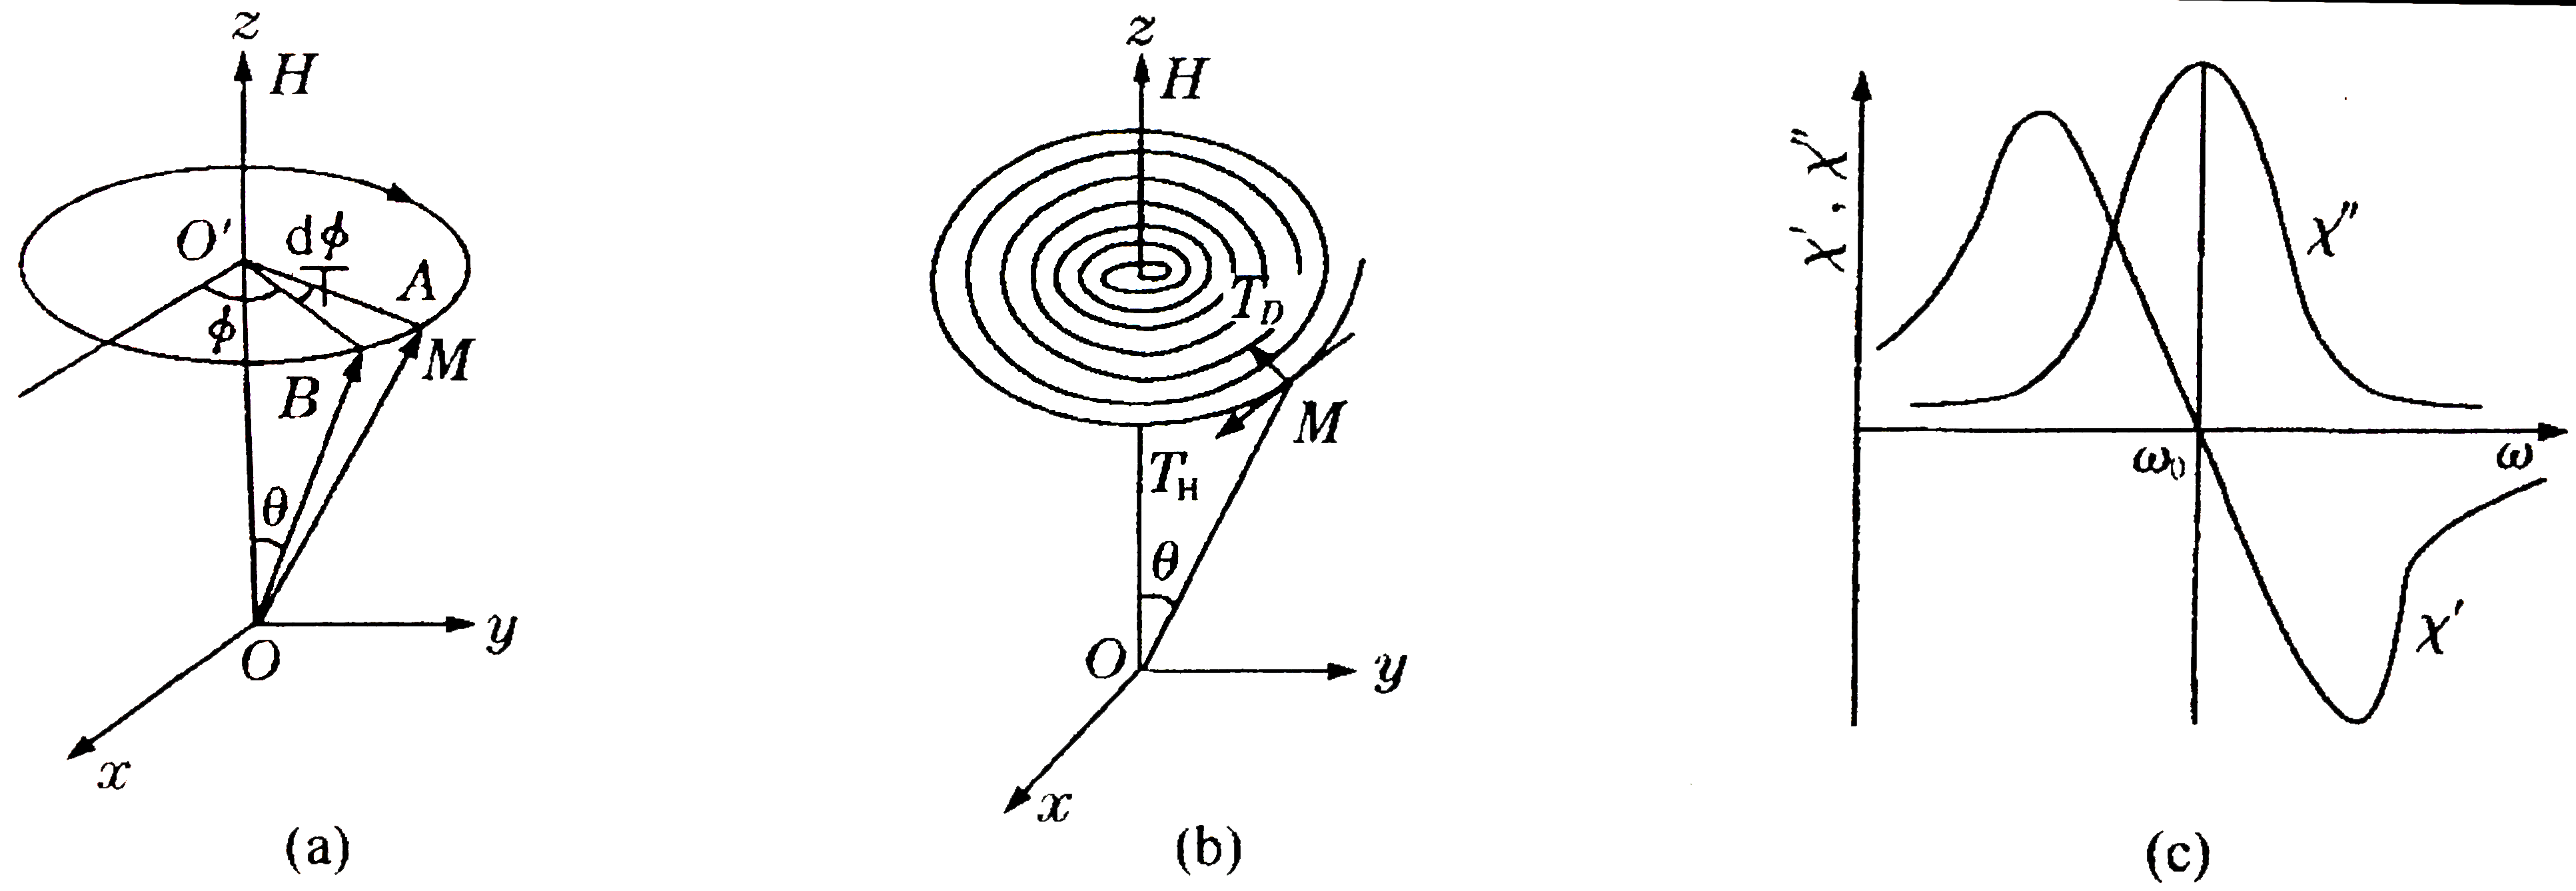
\includegraphics[width = \linewidth]{image/1.png}\\
\caption{原子核自旋磁矩在外磁场中的拉莫进动和核磁共振的经典描述}
\label{Fig1}
\end{figure}

在实际情况下,$\mathbf{M}$绕$\mathbf{H}$进动会受到阻尼作用,因而随着进动的进行,$\mathbf{M}$与$\mathbf{H}$之间的夹角$\theta$将随时间而减小,最后达到位置平衡,使$\mathbf{M}$平行于$\mathbf{H}$取向,如图\ref{Fig2}(a)所示,为了描述这一物理图像,可通过唯象地再同时引入一阻尼力矩$\mathbf{T}_D$,推导出下列进动方程:
\begin{equation}\frac{{\rm d}\mathbf{M}}{{\rm d}t}=\gamma\mathbf{M}\times \mathbf{H}+\mathbf{T}_D.\label{9.1-1}\end{equation}
阻尼力矩$\mathbf{T}_D$通常有三种表达式,即
Landau-Lifshitz形式:
\begin{equation}
\mathbf{T}_D=-\frac{4\pi\lambda}{M^2}\mathbf{M}\times (\mathbf{M}\times \mathbf{H})=-\frac{\alpha\gamma}{M}\mathbf{M}\times (\mathbf{M}\times \mathbf{H})\label{9.1-2}
\end{equation}

Gilbert形式:
\begin{equation}
\mathbf{T}_D=\frac{\alpha}{M}\mathbf{M}\times \frac{{\rm d}\mathbf{M}}{{\rm d}t}\label{9.1-3}
\end{equation}

Bloch形式:
\begin{equation}
\mathbf{T}_D=-\frac{M_x}{T_2}\mathbf{i}-\frac{M_y}{T_2}\mathbf{j}-\frac{M_z-M_0}{T_1}\mathbf{k}\label{9.1-4}
\end{equation}

以上公式中,$\lambda>0$,它是一个同阻尼力矩大小有关系的系数,量纲是时间的倒数,称为弛豫频率。$\alpha$是阻尼系数,$T_1$和$T_2$分别称为自旋-自旋(纵向)弛豫时间和自旋-晶格(横向)弛豫时间,通常,$T_2\le T_1$。在实际使用中,用Landau-Lifshitz形式处理自旋动力学问题时非常方便,因而使用最多,但是,当$\lambda$很大时,会出现矛盾。Gilbert形式在数学处理上最为简单,Bloch形式能对人体内所有核磁共振现象给出非常满意的描述,所以多在医学上讨论核磁共振原理和信号处理时被应用。

现在,考察一下核自旋系统在恒定磁场和交变磁场共同作用下的响应。如果沿$+z$方向施加一恒定磁场$\mathbf{H}_0$,沿$+x$方向施加一弱交变磁场$\tilde{h}=h_0{\rm e}^{j\omega t}$,且满足$h_0<<H_0$。将下列条件代入\ref{9.1-1}和\ref{9.1-2}式,得
$$\mathbf{H}=h_0{\rm e}^{j\omega t}\mathbf{i}+H_0\mathbf{k},$$
$$\mathbf{M}=m_{x0}{\rm e}^{j\omega t}\mathbf{j}+(M_0-m_{z0}{\rm e}^{j\omega t})\mathbf{k}$$
忽略二级小量,考虑到$h_0<<H_0$,近似有$\frac{{\rm d}m_z}{{\rm d}t}\sim0$,同时令$\omega_0=\gamma H_0$,$\omega_c=\frac{4\pi\lambda}{\chi_0}$,$\chi_0=\frac{M_0}{H_0}$,可得联立方程组如下:
\begin{equation}(\omega_c+j\omega)m_{x0}-\omega_0m_{y0}=\omega_c\chi_0h_0,\label{9.1-5}\end{equation}
\begin{equation}\omega_0m_{x0}+(\omega_c+jw)m_{y0}=\gamma M_0h_0.\label{9.1-6}\end{equation}
解方程,可得沿$x$轴方向的磁化强度分量为
\begin{equation}m_{x0}=\frac{\omega_c^2+\omega_0^2+j\omega\omega_c}{\omega_c^2-\omega^2+\omega_0^2+2j\omega\omega_c}\chi_0h_0.\label{9.1-7}\end{equation}
由此可以求得复数交流磁化率$\tilde{\chi}=\frac{m_{x0}}{h_0}$,如果将该磁化率写成$\tilde{\chi}=\chi'-j\chi''$,经整理可得该复量磁化率的实部和虚部的表达式:
\begin{equation}\chi'=\frac{(\omega_c^2+\omega_0^2)^2+\omega^2(\omega_c^2-\omega_0^2)}{(\omega_c^2-\omega^2+\omega_0^2)^2+4\omega^2\omega_c^2}\chi_0,\label{9.1-8}\end{equation}
\begin{equation}\chi''=\frac{\omega\omega_c(\omega_c^2+\omega_0^2+\omega^2)}{(\omega_c^2-\omega^2+\omega_0^2)^2+4\omega^2\omega_c^2}\chi_0.\label{9.1-9}\end{equation}
图\ref{Fig1}(c)示出了阻尼(即\ref{9.1-2}式中的$\lambda$值)很小时$\chi'$和$\chi''$随角频率$\omega$的变化关系。可以看到,当弱交变磁场的频率等于拉莫进动的频率即$\omega=\omega_0=\gamma H_0$时,$\chi'$发生从正值到负值的突变,而$\chi''$则达到峰值,这正好对应于核磁共振发生的情况。复数磁化率的物理意义在于其实部代表系统中储存的能量,而虚部则代表能量损耗。位于交变磁场中的单位体积原子核自旋磁矩系统将以一定速率从该磁场中吸收能量,每一周期$T=\frac{2\pi}{\omega}$中所吸收的能量为
\begin{equation}E=\mu_0\int_{t=0}^{t=T}\mathbf{H}\cdot{\rm d}\mathbf{M}.\label{9.1-10}\end{equation}
因为只有$h\frac{{\rm d}m_x}{{\rm d}t}$项对上式积分有贡献,因此,如果沿$x$方向的交变磁场写成$h=h_0\cos\omega t$,则$m_x$为复数意味着其实部和$h$同相位,而虚部落后于$h$的相位角为$\pi/2$,于是$m_x$可写成
\begin{align*}
    m_x&=\chi'h_0\cos\omega t+\chi''h_0\cos(\omega t-\pi/2)\\
    &=\chi'h_0\cos\omega t+\chi''h_0\sin\omega t
\end{align*}
代入\ref{9.1-8}式,积分后求得
\begin{equation}E=\pi\mu_0h_0^2\chi''.\label{9.1-11}\end{equation}
由此可知,单位体积核自旋系统每周从交变磁场中吸收的能量和交流磁化率的虚部成正比,图\ref{Fig1}(c)所示的$\chi''-\omega$关系反映了在实验上观察到的核磁共振峰的主要特点。

应该指出的是,在常见的核磁共振仪中,感生电动势是从一个垂直于交变磁场和恒定磁场放置的探测线圈中测得的。因此,实验时实际测量的是分量$m_y=m_{y0}{\rm e}^{j\omega t}$,从联立方程式\ref{9.1-5}和\ref{9.1-6}很容易求得
\begin{equation}m_{y0}=\frac{2\omega^2\omega_0\omega_c+j\omega\omega_0(\omega_c^2-\omega^2+\omega_0^2)}{(\omega_c^2-\omega^2+\omega_0^2)^2+4\omega^2\omega_c^2}\chi_0h_0.\label{9.1-12}\end{equation}

\subsection{}
氢原子核($^1$H)在有机化合物中占有很重要的地位。它对磁场的敏感度最大,容易观察到满意的核磁共振信号,因而目前对它的研究最多,应用也最广泛。

氢原子核只包含一个质子,自旋量子数为$I=1/2$,可以看成是电荷均匀分布于球面上的旋转椭球。在恒定磁场中,它有平行和反平行于磁场两种取向,相应于$m=+1/2$和$m=-1/2$。这两种取向的能量是不同的,用两个能级来表示,如图\ref{Fig2}所示。其中,$m=-1/2$能级因自旋取向与磁场方向相反,能量较高,这两个能级之间的能量差为
$\Delta E=\gamma_P\hbar H_0,$
式中,$\gamma_P=3.36166\times 10^2/$(A/M$\cdot$sec)是质子的旋磁比。

\begin{figure}[H]
\centering
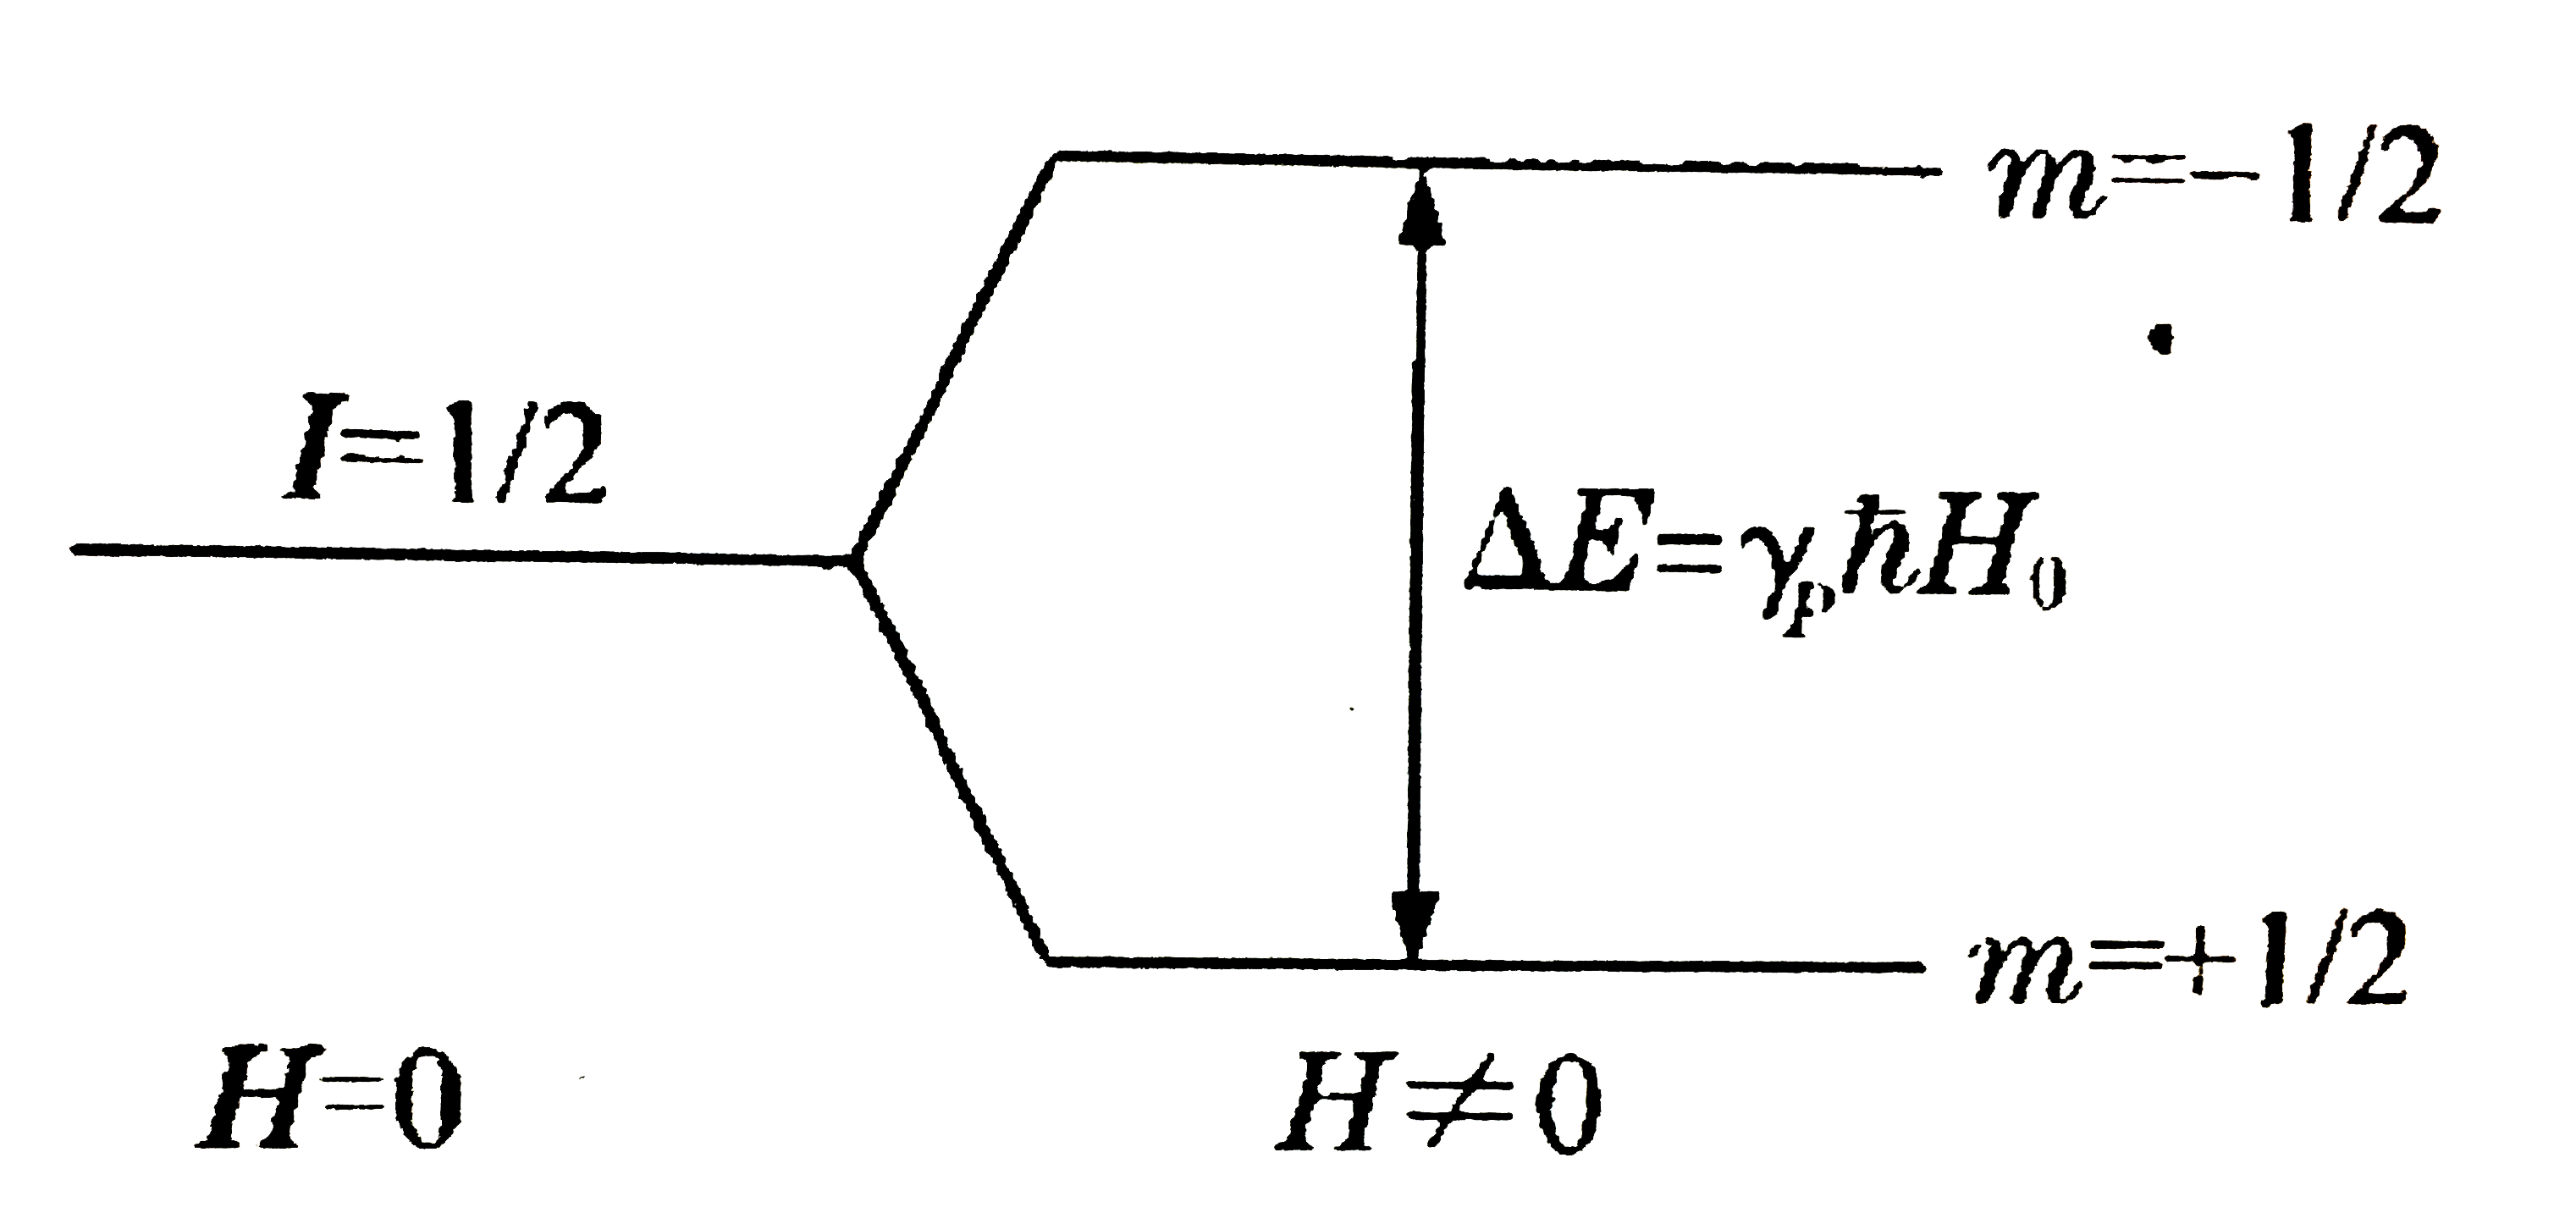
\includegraphics[width = \linewidth]{image/2.png}\\
\caption{氢原子自旋磁矩在恒定磁场中的能级分裂}
\label{Fig2}
\end{figure}

可由统计力学估算出热平衡条件下$m=+1/2$的质子数$N_+$与$m=-1/2$的质子数$N_-$之比:
\begin{equation}\frac{N_+}{N_-}=\exp\left(\frac{\Delta E}{kT}\right)=\exp\left(\frac{\gamma_0\hbar H_0}{kT}\right)\approx 1+\frac{\gamma_0 \hbar H_0}{kT}.\label{9.1-13}\end{equation}
假定$H_0=1.1214\times 10^3$kA/m(14902Oe),$T=300$K(这是60MHz核磁共振仪室温下测量的典型条件),则$N_+/N_-=1.0000099$,这就是说,在一百万个氢原子核中,热平衡条件下位于低能级的原子核数只比位于高能级的多10个左右。

如果要使位于低能级的核跃迁到较高能级去,即从$m=+1/2$的能级跃迁到$m=-1/2$的能级,就必须向原子核提供正好等于两个能级之间的能量差$\Delta E$的电磁波能量。如果在垂直于恒定磁场$H_0$的方向上对氢原子核系统施加一个角频率为$\omega_0$的交变磁场,其提供的能量$\hbar\omega_0$恰好等于$\Delta E$,就可发生使原先位于低能级的核跃迁到高能级去。于是从$\Delta E=\hbar\omega_0$
可得出发生核磁共振的必要条件为
\begin{equation}
\omega_0=\gamma_PH_0.\label{9.1-14}
\end{equation}

由此可知,所谓核磁共振,就是位于恒定磁场中的原子核持续不断地吸收弱交变磁场能量,从低能级跃迁到高能级的现象。由\ref{9.1-14}式可知,如果弱交变磁场的频率为60MHz,则当恒定磁场中为$H_0=1.1214\times 10^3$kA/m(14092Oe)时,氢原子核系统就可产生核磁共振。

如上所述,氢原子核在恒定磁场作用下,其原来兼并的能级分裂为二,由于占据低能级的核数稍大于占据高能级的核数,总的来说,仍有可能产生净的能量吸收现象。但是,两个能级上的核总数毕竟相差不大,再加上兆赫兹频率范围内氢核从高能级回到低能级的自发辐射的几率接近于零,因此,如果它们不能通过其他途径从高能级回到低能级,跃迁过程就会很快达到饱和而不再发生净的能量吸收,因而也就无法观察到核磁共振谱。幸好,这种非自发辐射的途径是客观存在的,称为弛豫过程。一是纵向弛豫,又称自旋-自旋弛豫,通过它,处于高能级的一核的能量被转移至处于低能级的另一核,但各种取向的核的总数保持不变。另一种弛豫是横向弛豫,又称自旋-晶格弛豫,经过这种过程,一些核由高能级回到低能级,同时将能量转移给周围的分子以热量的形式放出。正如前面所提到的,这两种弛豫过程相应的弛豫时间就是出现在\ref{9.1-14}式Bloch方程中的参数$T_1$和$T_2$。关于这两种弛豫过程的详细讨论,可参阅有关文献和著作。

在核磁共振实验中,除了外加的恒定磁场以外,还会在与恒定磁场相垂直的平面上
加上一个线偏振射频场,这个射频场可以看做是左旋圆偏振场与右旋圆偏振场的
叠加.在这两个场中,只有与磁化强度矢量做拉莫尔进动方向一致的射频场才会起
作用.

在伴随有效圆偏振射频场一起旋转的坐标系中解布洛赫方程式,便可以得到方程
的稳态解:
\begin{equation}
\begin{cases}
u = \frac{\gamma B_1 T^2_2(\omega_0 - \omega)M_0}{1 + T_2^2(\omega_0 -
  \omega)^2 + \gamma^2B_1^2T_1T_2}\\
v= \frac{-\gamma B_1 M_0T_2}{1 + T_2^2(\omega_0 -
  \omega)^2 + \gamma^2B_1^2T_1T_2} \\
M_z = \frac{\left[1 +T^2_2(\omega_0 - \omega) \right]M_0}{1 + T_2^2(\omega_0 -
  \omega)^2 + \gamma^2B_1^2T_1T_2}
\end{cases}
\end{equation}
其中$u$为$xoy$平面上磁化强度矢量与射频场磁场方向一致的矢量分量,相当于
动态复数磁导率的实部,称为色散信号;$v$为$xoy$平面上磁化强度矢量与射频
场磁场方向垂直的矢量分量,相当于动态复数磁导率的虚部,称为吸收信号.在实
验中,通过测量电路的不同处理方式,可以观察到色散信号或者吸收信号.

最后,通过对于吸收信号的形式分析,我们可以得到吸收谱线的半峰宽(FWHM:Full Width at Half Maxumum)为
\begin{equation}
\Delta \omega = \frac{2}{T_2}
\end{equation}
于是,通过测量吸收谱线的半宽度,我们可以测量材料的磁化强度矢量的横向弛豫
时间.

\section{实~~验}
实验装置的示意图如图~\ref{fig:ins}

\begin{figure}[htbp]
  \centering
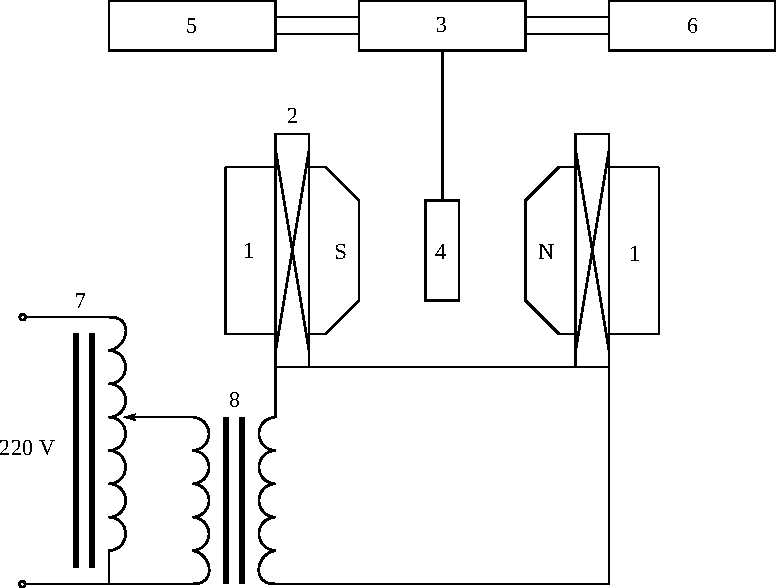
\includegraphics[width=\linewidth]{image/drawing.pdf}
\caption{\label{fig:ins}%
实验装置的方框图,图中各项为:1.永久磁铁~~2.扫场线圈~~3.电路盒~~4.样品和
振荡线圈~~5.数字频率计~~6.示波器~~7.可调变压器~~8.220V/6V变压器
}
\end{figure}

\subsection{固定磁场}

本实验的固定磁场由永久磁铁提供$B_0 > \SI{0.5}{T}$,在均匀区
$(\SI{5}{mm})^2$范围内均匀性优于$\num{1e-5}$, 稳定性:五年内变化<0.05\%, 磁极直径:65mm,磁隙宽度:大约13mm,可以满足核磁共振实验的相应要求.

\subsection{射频磁场}

射频磁场由电路盒中的振荡电路通过振荡线圈产生,产生的磁场是线偏振的射频
磁场.如前文所述,该线偏振射频场可以看作两个旋转方向相反的圆偏振磁场的叠
加,而其中的有效射频场只有一个.

\subsection{接收电路}

我们采用单线圈法,振荡线圈既是发射线圈,也是接收线圈.电路盒中采用边限振
荡器作为测量电路.边限振荡器在调节适当的情况下,不会工作在稳定
状态,而是工作在刚刚起振的边缘状态,此时任何电路参数的改变都会引起工作状
态变化.当共振发生时样品要吸收射频场能量,使得振荡线圈$Q$值减小,导致振荡
器工作状态改变,表现在振荡波形包络线发生变化,该信号经检波、放大处理
后,从电路盒背面的"检波"端口输出,在示波器上即可观察到共振吸收信号.

\subsection{扫~场}

实验采用扫场的方式观察核磁共振吸收信号,即通过改变磁场$B_0$的大小,来改
变$\omega_0$的值,从而改变$\omega-\omega_0$这一相对值的大小,进而实现对
于核磁共振吸收信号的观测.

\subsection{实验过程}
实验首先通过测量掺有 \sFeCl3 的 \sHIIO 样品中的质子共振信号,为装置中的永久磁铁磁场定标。

然后调频使得共振先后发生在扫场的波峰和波谷,此时相邻的共振信号间隔变为20ms,测量得到扫场的幅度。共测量五组数据。利用 $B_0= \frac{\nu_H}{\left( \gamma\2\pi \right)_H}$得到磁场强度,$\DeltaB_0= \frac{\left(\nu_H^{'} - \nu_H^{''}\right)}{\left( \gamma\2\pi \right)_H}$得到误差范围。

同时左右移动水样品的电路盒测量磁场边缘的磁场强度并与中心的磁场强度比较。得到一组数据。

实验接下来通过测量"聚四氟乙烯"样本中的原子核共振信号, 利用 $g=\frac{\nu_F / B_0}{\mu_N /h}$ 测量了氟原子核的
$g$因子,$\frac{\Delta g}{g}=\sqrt{\left(\frac{\Delta \nu_F}{\nu_F}\right)^2+\left(\frac{\Delta B_0}{D_0}\right)^2}$ .得到五组结果。

实验最后改用X-Y输入方式,利用 $1/T_2=\pi \Delta B(\gamma/2\pi)_H$ 估测了"聚四氟乙烯"样品的横向弛豫时间,测得这一样品的共振峰半峰宽(FWHM).

\enlargethispage{-3.3cm}


\section{实验结果与分析}
实验的所有直接测量结果见表~\ref{tab:rawdata}.

\begin{table}[t]
\caption{
\label{tab:rawdata}%
实验的直接测量数据表.表中的共振频率 $\nu_H$ 为在示波器上观察到明确核磁共振吸收
信号的对应频率;上限共振识别频率 $\nu_H^'$ 与下限共振识别频率 
$\nu_H^{''}$ 为调节射频场频率时,刚
好使得共振信号不可识别的最大和最小频率,用于计算测量的误差.}

\begin{ruledtabular}
\begin{tabular}{llll}

样品 & $\nu_H$/MHz & $\nu_H^'$/MHz & $\nu_H^{''}$/MHz \\ \hline
水 & 24.880 & 24.853 & 24.901 \\
 &24.895&24.866&24.924\\
 &24.874 &24.857&24.888\\
 &24.874&24.845 &24.900\\
 &24.880 &24.851&24.909\\
移动水样品 &24.872 &24.843&24.899\\
 
聚四氟乙烯 & 23.393 & 23.260 & 23.524\\
&23.388&23.255&23.522\\
&23.394&23.260&23.524\\
&23.389&23.254&23.524\\
&23.385&23.253&23.520
\end{tabular}
\end{ruledtabular}

\end{table}

质子的回旋频率为\cite{qian}

\begin{equation}
\frac{\gamma}{2\pi} = \SI{42.5763888 \pm
  0.0000018}{MHz/T}
\end{equation}

计算得到永久磁铁磁场的测量值应为
\begin{equation}
B = \SI{0.5843 \pm 5.871801e-5}{T}
\end{equation}

取玻尔磁子为\cite{qian}
\begin{equation}
\frac{\mu_N}{h} = \SI{7.62259396 \pm 0.00000031}{MHz/T}
\end{equation}

计算得到氟原子核的$g$因子测量值应为
\begin{equation}
g = \num{5.2512 \pm 0.00009}
\end{equation}

半峰宽与扫场范围之比为: $\frac{\Delta B}{2B^{'}}=0.5/6.137$ ,结合上文测得扫场范围测得这一样品的共振峰半峰宽(FWHM)为
\begin{equation}
\Delta B = \SI{9.5679e4}{s^{-1}}
\end{equation}
计算得到估测的横向弛豫时间.
\begin{equation}
T_2 \approx \SI{7.818e-8}{s}
\end{equation}




\section{结~~论}
本实验得到了掺有 \sFeCl3 的 \sHIIO 样品中质子的核磁共振信号,由此验证了核磁共振现象;在此基础上,实验中利用\specWaterPlus 样品质子共振信号和质子回旋频率的参考值对永久磁铁的磁场进行了校准;并进一步利用校准后的磁场测定了氟核的$g$因子,大约为 $g = \num{5.2512 \pm 0.00009}$ 。

此外,通过估测信号的半宽度$\DeltaB$, 估测了聚四氟乙烯中氟核的横向弛豫时间,大约为 $T_2 \approx \SI{7.818e-8}{s}$ 。


%%%%%%%%%%%%%%%%%%%%%%%%%%%%%%%%%%%%%%%%%%%%%%%%%%%%%%%%%%%%%%%%
%  参考文献
%%%%%%%%%%%%%%%%%%%%%%%%%%%%%%%%%%%%%%%%%%%%%%%%%%%%%%%%%%%%%%%%
%  参考文献按GB/T 7714-2015《文后参考文献著录规则》的要求著录. 
%  参考文献在正文中的引用方法:\cite{bib文件条目的第一行}
\section{参考文献}

[1]钱建强, 张高龙. 近代物理实验[M]. 北京航空航天大学出版社, 2016.
% \renewcommand\refname{\heiti\wuhao\centerline{参考文献}\global\def\refname{参考文献}}
% \vskip 12pt

% \let\OLDthebibliography\thebibliography
% \renewcommand\thebibliography[1]{
%   \OLDthebibliography{#1}
%   \setlength{\parskip}{0pt}
%   \setlength{\itemsep}{0pt plus 0.3ex}
% }

% {
% \renewcommand{\baselinestretch}{0.9}
% \liuhao
% \bibliographystyle{gbt7714-numerical}
% \bibliography{./TempExample}
% }


\end{document}
